\section{Introduction}

\vspace{-2mm}

Facial expression editing aims to transform the facial expression in an input image into a specific target expression while preserving other elements of the image, such as the person's attributes and background information~\cite{ding2017exprgan}. This task has widespread applications in human-computer interaction, gaming, and animated films, attracting considerable attention from the academic and industrial communities~\cite{melnik2024face}. With the development of diffusion models~\cite{dhariwal2021diffusion, ho2020denoising, sohldickstein2015deep}, significant progress has been made in the field of image synthesis and editing. Although diffusion models are renowned for their flexibility in handling various modalities such as texts and segmentation masks, challenges remain in facial expression editing, such as maintaining consistency in non-expression areas with the input~\cite{ling2020toward}. Currently, most expression editing techniques require explicitly specifying the target expression, typically through a conditional image or one-hot vector, lacking flexibility and failing to leverage the power of large language models~\cite{ling2020toward,ding2017exprgan,li2023reganie}. Our proposed research method utilizes natural language contexts, enabling the model to predict the appropriate facial expressions of the characters in the input picture based on the understanding of the scene or event contexts and to accomplish natural and accurate editing of facial expressions.
\vspace{-2mm}

\section{Methodology}

\vspace{-2mm}

We first develop a baseline pipeline capable of end-to-end understanding of context scenes, inferring character expressions, and editing the original image's facial expressions based on ControlNet~\cite{zhang2023adding}. Our overall framework is depicted in Fig.\ref{fig:framework}. Our method's inputs include: 1. A natural language description of the scene or event. 2. A target individual's facial image (not necessarily a close-up of the face, but reducing background information indeed helps lower the difficulty). Compared to the original ControlNet, we consider no prompt text or few static attributes and background descriptions as prompt text input. We allow the large model to predict the character's possible expressions in the current context and process the input text description into a new prompt text, guiding an Stable Diffusion model to generate a close-up image of the character's face with the target expression. Subsequently, we perform facial landmark detection~\cite{bulat2017far} on this close-up to obtain a facial landmark image containing expression information, which is also the input condition image for ControlNet. Following this, we train the model according to ControlNet's fine-tuning method~\cite{landmark}.

\begin{figure}[h!tp]
    %\centering
    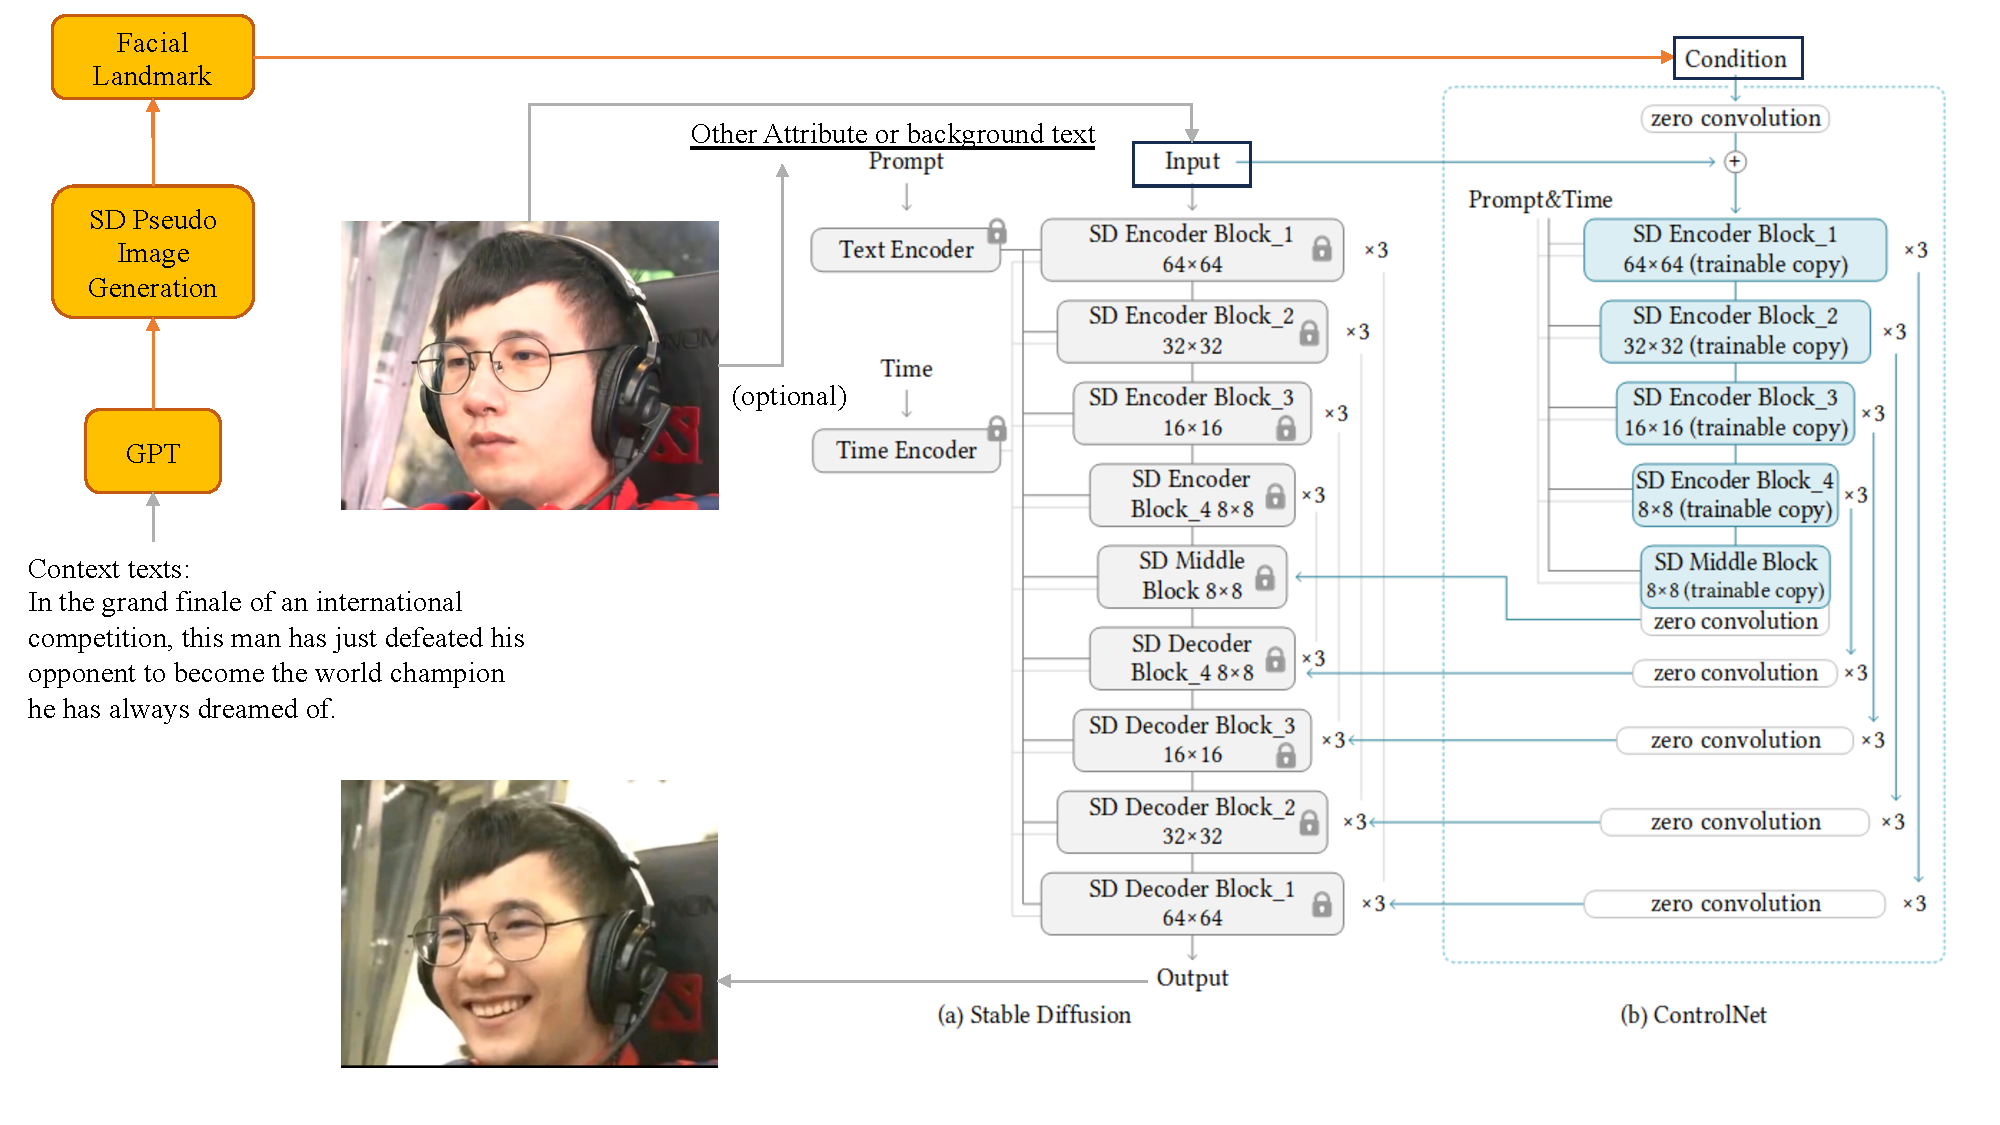
\includegraphics[width=1.3\linewidth]{figs/baseline_framework_proposal.pdf}
    \caption{The Overview of our baseline method. Use LLM to understand the given context settings, and deduce the proper facial landmark based expression information as condition control. Fine-tune the ControNet, enabling precise tailoring of facial expressions.
    }
    \label{fig:framework}
\end{figure}

\vspace{-5mm}


% Face generation and editing models, such as StyleGAN~\cite{karras2019style}, have been a powerful booster for gaming, animation, advertising, art and many other real-world applications~\cite{melnik2024face}. 

% We plan to build a better face expression editing model based on ControlNet~\cite{zhang2023adding}. 

% \section{Related Work}
% \cite{huang2023collaborative}
% \cite{ding2017exprgan}
% \cite{ling2020toward}

% Control the face expression by a landmark image: ~\url{https://huggingface.co/georgefen/Face-Landmark-ControlNet}



\section{Datasets}
\vspace{-2mm}
\textbf{AffectNet Dataset}~\cite{Gera_2021} is a large facial expression dataset with around 0.4 million images manually labeled for the presence of eight (neutral, happy, angry, sad, fear, surprise, disgust, contempt) facial expressions along with the intensity of valence and arousal.

\textbf{The Oulu-CASIA NIR\&VIS facial expression database}~\cite{4761697} consists of six expressions (surprise, happiness, sadness, anger, fear and disgust) from 80 people between 23 and 58 years old.

Based on the above available datasets, we will use manual crafting or CLIP-based heuristic method to construct context-expression image pair as our final training data.

\section{Evaluation}
\vspace{-2mm}
In this research, we apply same evaluation settings as in ~\cite{zhang2023adding}, including Network-based Metrics and Human-based Metrics.

\section{Timeline}

\noindent\begin{tabular}{|m{3cm}|m{12cm}|}
\hline
\textbf{date} & \textbf{event} \\
\hline
20240331 & Dataset Preparation and Test ControlNet Demo \\
\hline
20240410 & Framework Implementation \\
\hline
20240430 & Experiments and Try Possible Improvements \\
\hline
\end{tabular}